\documentclass[preprint,authoryear,12pt]{elsarticle}
\PassOptionsToPackage{hyphens}{url}\usepackage{hyperref}
\usepackage{amssymb}
%\usepackage{amsmath}
\usepackage{pslatex}
\usepackage[overlap,CJK]{ruby}
\usepackage{linguex}
%\usepackage[pdftex]{graphicx}
\usepackage{graphicx}
\usepackage{multirow}
\usepackage{subfigure}
\usepackage{paralist}
%\usepackage{setspace}

\newcommand{\hlc}[2][yellow]{ {\sethlcolor{#1} \hl{#2}} }

\renewcommand{\baselinestretch}{1.5}
\date{}
\pagestyle{empty}

\usepackage{color}
\usepackage{soul}

 \topmargin0mm
 \headheight0mm
 \headsep0mm
 \oddsidemargin0cm
 \textwidth15.5cm
 \textheight23cm

%% a useful little macro for comments and notes
\newcommand{\MNOTE}[1]{\marginpar{\tiny\raggedright\em #1}}
\setlength{\marginparsep}{2.2pt}
\setlength{\marginparwidth}{40pt}
%%\newcommand{\MNOTE}[1]{}
\newcommand{\Dutchvon}[2]{#2}

\setcounter{secnumdepth}{4}
%\newcommand{\comment}[1]{{\color{blue}{#1}}}
%\newcommand{\commenthp}[1]{{\color{red}{#1}}}
%\newcommand{\subsubsubsection}[1]{\paragraph{#1}\mbox{}\\}

\makeatletter
\renewcommand{\paragraph}{\@startsection{paragraph}{4}{\z@}%
  {-3.25ex\@plus -1ex \@minus -.2ex}%
  {1.5ex \@plus .2ex}%
  {\normalfont\normalsize\mdseries}}
\renewcommand{\subparagraph}{\@startsection{subparagraph}{5}{\z@}%
  {-3.25ex\@plus -1ex \@minus -.2ex}%
  {1.5ex \@plus .2ex}%
  {\normalfont\normalsize\bfseries}}
\makeatother


\begin{document}

\begin{frontmatter}
\title{Large-Scale Data Collection of Eco-Driving Behavior:
Analysis of a Campaign with the iCO$_2$ Simulation Platform}

\author[label1]{Helmut Prendinger}
\author[label2]{Henrique T. Campos}
\author[label2]{Hugo M.C. Damas}
\author[label1]{Anjie Fang}
\author[label1]{Zhi Qu}
\author[label1]{Bernd Hollerit}
\author[label2]{Rui Prada}


%\author[label3]{Klaus Br\"ugmann}

\address[label1]{{helmut@nii.ac.jp, fanganjie@gmail.com, hollerit@gmail.com, zq12721@my.bristol.ac.uk}\\
	National Institute of Informatics, \\
    2-1-2 Hitotsubashi, Chiyoda-ku, Tokyo, 101-8430, Japan\\}

\address[label2]{{henriquetcampos@gmail.com,hugo.damas@gmail.com,rui.prada@tecnico.ulisboa.pt}\\
    INESC-ID and Instituto Superior T\'{e}cnico, Universidade de Lisboa,\\
    Av. Prof. Cavaco Silva, Taguspark Porto Salvo, Portugal\\}

%\address[label3]{{mail@klausbreugmann.de}\\
%	??? \\
%	Tokyo, Japan\\}

\begin{abstract}
We describe iCO$_2$, a simulation platform for collecting driving behavior data. For the user, iCO$_2$ is designed as a massively multiplayer online game for mobile devices to practice eco-friendly driving. For the researcher, iCO$_2$ constitutes a Human Computation system that facilitates the collection of large-scale data on driving behavior to better understand incentive mechanisms for eco-driving and users' preferences. The main contribution of the paper is two-fold. First, we describe the newest version of our iCO$_2$ simulation platform, which has been extended to a game with a quest system and functions to upgrade the player's vehicle. Second, we present the results of a campaign with iCO$_2$ that uses a game promoter to attract more than 3000 users in a short time. Our game run on servers in Asia, Europe and America. The results are described in terms of users' interaction with game elements and clustering of driving behavior. The novelty of the paper relates to the insights gained from analyzing driving behavior and preferences of users attracted via a mobile game promoter.
\end{abstract}

\begin{keyword}
Data collection; data analysis; driving behavior; Human Computation system; Games with a Purpose; massively multiplayer online game
\end{keyword}

\end{frontmatter}

%%%%%%%%%%%%%%%%%%%%%%%%%%%%%%%%%%%%%%%%%%%%%%%%%%%%%%%%%%%%%%%%%%%%%
% INTRODUCTION
%%%%%%%%%%%%%%%%%%%%%%%%%%%%%%%%%%%%%%%%%%%%%%%%%%%%%%%%%%%%%%%%%%%%%
\section{Introduction and Motivation}\label{sec:intro}

%Testing references:
%\citep{Andrade+others.2005,Bellotti+others.2009,Hwang+Salvendy.2010,Csikszentmihalyi.1990}
%\cite{Andrade+others.2005,Bellotti+others.2009,Hwang+Salvendy.2010,Csikszentmihalyi.1990}

Our world today is tightly interconnected by the Internet, which allows users from almost anywhere to access information anytime in an affordable and immediate manner. For scientists, this situation opens hitherto unknown opportunities for experimental testing of novel online applications. While in principle vast populations can  be reached quickly and effortlessly, motivating users to participate in social experiments is a big challenge. It is important to provide an adequate incentive other than money to the users, so that they do not have any motivation to cheat \citep{Quinn}.
As a solution, Games With a Purpose (GWAP) have been proposed \citep{vonAhn2006Games}. GWAP is a field of Human Computation \citep{Yuen.2009,Krause+Smeddinck.2011} that seeks to motivate users, such as annotators of pictures or testers of applications, through enjoyment rather than any monetary incentive.

The recent rise of mobile devices---such as smart phones, tablet computers or handheld game consoles---
%has rendered traditional lab studies impractical. 
\hlc[green]{
has opened up new opportunities to conduct experiments beyond laboratory studies. This ubiquitous computing makes it possible to reach large numbers of users, however it also makes it more difficult to standardize test conditions, and control the environment.}
Researchers have suggested a ten-step-program to conduct large-scale studies with mobile applications in order to obtain valuable data that cannot be collected in a lab setting:
\begin{inparaenum}[\itshape 1\upshape)]\item Clearly identify the research goals; \item Select a study method; \item Devise an incentive mechanism;  \item Choose the target platform(s); \item Design and develop the mobile app; \item Prepare data collection; \item Implement a scheme to obtain informed consent from users; \item Distribute and promote the app; \item Continuously monitor data collection for a designated time period; \item Filter and analyze data to answer the research question \end{inparaenum} \citep{Henze2013}.

In this paper, we broadly adhere to these steps and present iCO$_2$, a massively multiplayer online (MMO) driving game designed as a mobile application that allows players to practice eco-friendly driving. Notably, iCO$_2$ is a platform for collecting driving behavior data and in-game decision data from users. It can be accessed as an app on ``Google play''.\footnote{https://play.google.com/store/apps/details?id=net.globallabproject.ico2\&hl=en}
Our data collection platform uses a hybrid strategy to give an incentive to players, which is \begin{inparaenum}[\itshape a\upshape)] \item based on a mobile games promoter to attract players to the game and \item in-game mechanics to keep them playing. \end{inparaenum} We use Tapjoy\footnote{http://home.tapjoy.com/}, %\citep{TapJoy}
a company that handles mobile games promotion, to attract a large number of users (in the 1000s) to iCO$_2$ within a short time. This approach constitutes an alternative to the tools and applications that have been used in research projects involving games \citep{kittur2008crowdsourcing,Biewald:2012,ChanH12}.
In order to keep players motivated, we provide a quest system and the possibility to upgrade the user's car as in-game mechanics.

The main contribution of this paper is a human-computer study that aims to help us understand how users interact with a mobile game on eco-driving, 
\hlc{[green]}{and the way their driving style evolve.} 
Since we built our own multiuser game, we had full access to all the behavior data of the users. We could obtain unique insights into the users' activities in terms of eco-driving types (eco-friendly, normal, etc.) and the usage of the ``garage'', where users could upgrade and modify their car with the in-game money rewarded from the quests. Our study is exploratory as it was difficult to formulate hypotheses on users' behavior beforehand. However, its results allow one to improve the design of the game.

%Our great objective is to collect real-time accurate big data, data that is to framed into a knowledge base relevant to eco-driving, which is why we also show and discuss how big a step iCO$_2$ has taken towards the smaller objective of helping individuals understand, and practice, eco-friendly driving in a more accessible and still relevant manner. Current technologies either involve linear 2D applications \citep{EcoGame1,EcoGame2,TruckEcoGame,Moebius,FiatEcoGame}, or driving simulators that must be played on the respective physical chair-wheel-and-pedals simulator \citep{EcoSimulator,GreenDino,EcoSimulator2,sabrina2013enhanced} or support applications or mini-games that focus on relevant information feedback \citep{FiatEcoGame,EcoTools,Brunnberg04theroad,endres2010youldeco}.

%Managing a massively multiplayer application is very difficult work, as is acquiring users to participate in a serious game or a human computation system, but as we hope to demonstrate, iCO$_2$ has made good progress on all fronts and has definite potential for meaningful data retrieval and processing on a yet-unmatched scale.

\hlc[green]{
	This paper is structured as follows. }
Section \ref{sec:background} 
\hlc[green]{provides background research on eco-driving games, training applications, crowdsourcing and games with a purpose. 
}Section \ref{sec:platform} 
\hlc[green]{describes the iCO$_2$ simulation platform, which extends our previous version of iCO$_2$
}\citep{prendingeroliveira2014} 
\hlc[green]{with a quest system and upgrade functions. THIS IS A TEST 
	On Section 
}
\ref{sec:campaign} 
\hlc[green]{we provide insights obtained from the data collected from a user acquisition campaign. Besides overall statistics (presented in Section 
}
\ref{subsec:usage_stats}), 
\hlc[green]{we try to find patterns in the driving behavior using clustering methods
}(Section \ref{subsec:clustering}), 
\hlc[green]{we also mention other behavioral data insights. Moreover we test, and discuss whether our hypothesis in which iCO$_2$ players tend to become better at eco-driving (by considering smooth acceleration and brakings), the longer they play, on Section
}
\ref{subsec:eco-friendliness_over_time}.
Section \ref{sec:conclusions} 
\hlc[green]{concludes the paper, by summarizing and discussing the most relevant results while paving the way for future work.}

%The appendix contains additional tables in \ref{app:tables} and the list of abbreviations in \ref{app:abbreviations}.

%%%%%%%%%%%%%%%%%%%%%%%%%%%%%%%%%%%%%%%%%%%%%%%%%%%%%%%%%%%%%%%%%%%%%
% RELATED WORK
%%%%%%%%%%%%%%%%%%%%%%%%%%%%%%%%%%%%%%%%%%%%%%%%%%%%%%%%%%%%%%%%%%%%%	
\section{Related Work}\label{sec:background}

We will first report on eco-driving games and training applications and analyze how iCO$_2$ differs by involving a massively multiplayer element, a mobile distribution method and a three dimensional (3D) environment.
Then we will explain how our work can be positioned within the crowdsourcing literature.

\subsection{Eco-driving Games and Training Applications}
\label{subsec:eco-driving}

\hlc[green]{
Eco-driving is a term used to describe the usage of vehicles in an energy efficient way. The main objective is the reduction of fuel consumption, so that the same amount of fuel allows for a longer mileage.
}
The training of eco-driving is important as it greatly affects world-wide fuel expenditure and pollution emissions \citep{barkenbus2010eco,shaheen2012ecodriving}. Therefore, car manufacturers are starting to develop applications that provide drivers with some feedback on the effects of their driving behavior \citep{EcoTools,FiatEcoGame}.

iCO$_2$ is first and foremost an eco-driving game. It has been designed to work as a massive multiplayer online (MMO) game. Therefore it is possible that users interact with each other, as they would in real life driving. It has been designed to be played in mobile systems so that it is as  accessible as possible by the masses. In particular, our target audience are gamers; a group that has seen its size and playtime exponentially grow over recent years \citep{MobileStats}.

It is important to note that the player is not the only one who receives feedback on his or her  driving. Our underlying data gathering system can provide important information to future developers of iCO$_2$ on how to improve the design of the eco-driving simulator.

The aforementioned qualities make iCO$_2$ stand out from any other eco-driving application in the industry.
We have observed that applications that allow users to practice eco-friendly driving and to learn the impact that their performance has on their fuel consumption or gas emission are either 2D single-player games (\cite{EcoGame1, EcoGame2, TruckEcoGame, Moebius, FiatEcoGame}) or full-fledged simulators that can only be played with specific physical apparatus (\cite{EcoSimulator, GreenDino, EcoSimulator2, sabrina2013enhanced}).

While there are MMO driving games, none of them allows users to keep track of the effect of their driving behavior on their fuel consumption and gas emissions. And while there are applications, even games, which incorporate the aforementioned features, none of them are MMO driving games.

\subsection{Crowdsourcing and Games with a Purpose}
\label{subsec:csandgwap}

We have defined our project as a Human Computation system \citep{Yuen.2009,Krause+Smeddinck.2011}, and not as a crowdsourcing system. \cite{Quinn} explain the difference comprehensively --- the most important distinction is that crowdsourcing involves the entire problem being tackled by a crowd of humans \citep{howe2008crowdsourcing}, while Human Computation involves only part of a problem being tackled by a crowd of humans.

Our goal is to collect and discern driving behavior. Our users fill in for a part of the ``algorithm'' of data collection, which involves them ``providing behavior''. 
%Our game neatly adheres to the definitions of Games With a Purpose given by \cite{Quinn} and \cite{vonAhn2006Games}, albeit with a slightly more ambiguous problem definition: to collect real-time behavioral driving data from users.
We consider our game fits the definition of Games With a Purpose given by \cite{Quinn} and \cite{vonAhn2006Games}, which is explained as an area in the field of Human Computation that aims to use enjoyment as a primary means of motivating users. The main purpose of iCO$_2$ is the data collection of real-time behavioral driving data from users, who are encouraged to drive in an eco-friendly way. The longer our system can keep the players interested, the more behavioral data we will be able to capture. 



Our method to provide the system with users is based on Tapjoy. Despite our system being focused on the enjoyment of players as the main strategy to motivate users to play through the game, we initially provide a monetary incentive, akin to other mobile games, to get the users into our system for the first time. Tapjoy works by offering mobile gamers in-game rewards for whatever game they are playing, in exchange for engaging with another game up to a specific requirement. In our experiment (see Section~\ref{sec:campaign}), we motivated users to try our game in that way: Tapjoy requires them to spend a certain amount of time in the game environment, after which only the enjoyment factor could keep them engaged.
As mentioned in Section~\ref{subsec:eco-driving}, our game is an MMO, potentially involving a massive level of player interaction, which, in addition to the aforementioned characteristics, sets iCO$_2$ apart from other Games with a Purpose, as well as other crowdsourcing systems.


\subsubsection{Crowdsourcing}

\cite{Biewald:2012} and \citep{ChanH12} introduce systems that might be related to ours; however, they do not involve GWAP. Biewald presents a number of applications involving crowdsourcing and Human Computation, notably using the increasingly popular Mechanical Turk from Amazon \citep{MechTurk}, involving ethics, business and fun, putting a crowd of people to work immediately on simple tasks. These tasks involve answering questions that don't require any technical knowledge and performing Google searches. ``Sifu'' by \citep{ChanH12} is a system that supports language learning by providing tutoring services to readers of news sites and articles. Crowd members are recruited from an online social network instead of using the Mechanical Turk.

We note that while these two applications use distinct sources of ``crowds for hire'', they are acquiring a group of users to participate in their research by performing specific tasks that constitute the experiment as a whole. This further illustrates why we consider iCO$_2$ a Human Computation system: iCO$_2$ is not meant to rely on hiring a crowd to do a (particular) job, but rather to play a game, have fun and practice eco-driving. As a side effect, the crowd will be providing reliable data about their behavior in an accessible manner, which is our target effect. However, our intended goals don't necessarily motivate the crowd of users. This is where Games with a Purpose come into play.

\subsubsection{Games with a Purpose}

iCO$_2$ is a Game with a Purpose: data collection. In particular, we are interested in driving behavior data, which constitutes a higher level purpose compared to other approaches. Considering this, we will contrast our project to other GWAPs that have been involved in research endeavors.

%\paragraph*{Image tagging -- ESP game, Peekaboom, Phetch, KissKissBan, Karido}

Von Ahn et al. introduced the concept of GWAP with the now well-known ESP game \citep{vonAhn:2004}. Its purpose was to label images: players are matched one to one to try and guess which label their competitor is applying to the image that both of them are seeing. Subsequently, the project was improved and re-branded as Peekaboom \citep{vonAhn:2006} and Phetch \citep{vonAhn:2007}.

KissKissBan \citep{Ho:2009} extended on previous approaches of player matching by integrating cooperative and competitive elements into a game with the purpose of annotating images. One player tries to make it so a pair of other players can't agree on a description about an image, which not only adds a cheating-proof mechanism but also promotes diversity of image annotations. Even later, these concepts were extended with more functionality by another team with their game Karido \citep{steinmayr2011karido}.

All of these applications are successful in improving image databases, focusing on labeling, description, information (knowing what objects an image contains), and keyword/tag diversity (by providing similar images, so users are forced to choose differentiating keywords/tags), respectively. However, in all of them, even with being played by a massive crowd of players, user interaction is always on a small scale: one to one.

%\paragraph*{Audio tagging -- TagATune}

A similar approach to the previously outlined image tagging endeavors is taken with TagATune \citep{Law:2009}, a game with a purpose that also matches players online one to one. They play a game of tagging a piece of music that may or may not be shared by the two and when they are offered each other's music and tags, they try and guess if it is indeed the same sound sample or not. The game resurfaced with the modified intent of gauging the success of machine-run algorithms that tag music \citep{vonAhn&Law:2009}.

%\paragraph*{User preference -- Matchin}

Matchin \citep{Hacker:2009} is a GWAP that follows the same gameplay flow as ESP but instead of tagging, each player has two images and has to try and guess which one will be preferred by the matched player. The goal is to gather information on user preference for an image database.

%\paragraph*{Location tagging -- EyeSpy}

EyeSpy \citep{Bell:2009}, more of a social networking endeavor, motivates players to tag locations with descriptions, and then others to confirm them, by having a point system and a ranking. Meanwhile, the system retrieves a collection of recognizable geographic details that can be used towards supporting navigation tasks. Notably, EyeSpy is available on web-browsers and mobile applications, akin to iCO$_2$.

%\paragraph*{Collecting common sense facts \& goals -- Verbosity, CommonConsensus}

Verbosity \citep{vonAhnVerb:2006} and CommonConsensus \citep{lieberman2007}, while having different purposes, are both web-based knowledge games where players play via the browser to select an answer to given questions that is considered more or less correct. They are given a question and choose an answer they expect strangers to give. The more frequently an answer is given, the more correct it is considered. There is no user-to-user interaction in the case of these two applications besides interacting with the knowledge produced by the masses (which includes them). Verbosity sought to collect facts that were commonsense while Common Consensus sought to collect goals.

%\paragraph*{Prediction of protein structures -- Foldit}

Foldit \citep{cooper2010predicting} puts players in a puzzle-solving game involving the prediction of protein structures. By providing online functionalities such as chatting or ranking, they keep their players engaged with both difficulty and socialization. Chatting and ranking are functionalities iCO$_2$ does not provide at this point, because we believe those features would distract from the core functionality and purpose of the game.

%\paragraph*{Behavioral data -- Caretaker}

Caretaker \citep{Violi:2011} is a project that notably focuses on behavioral data, and the analysis thereof, that pertains to trust. Caretaker places four players in a board-like game that simulates a transport square-shaped network across which they have to travel from corners to center. Three players must ally against the fourth and arrive at the center before this common enemy, despite none of the three knows who the adversary is when the game starts. Their position in the network is the only publicly available information but the game offers a chat system to communicate as they wish. Violi et al. also logged player actions as a method through which they can match and confirm the behavioral information they receive from having the players submit a survey.

\paragraph*{Comparison of previous Games with a Purpose to iCO$_2$}

Caretaker has many similarities to iCO$_2$ as a Human Computation system: the player's actions and decisions are logged in order to analyze behavioral data.
%and the users are playing with and against each other, which approximates real behavior. However, we posit that the goal of the ``bad'' player is to be the enemy of the other three, while the goal of the other three is to find out who their friends are. If they know who is who, they can cooperate to win.
In iCO$_2$, the situations are potentially much more akin to real life circumstances, with drivers just encountering other motorists they know nothing about, and choosing how to interact with them based on the same variables that would influence them in a real scenario (situation, mood, etc). There is also the massive multiplayer element to iCO$_2$, which Caretaker does not have.

%When regarded as a whole, there is no research project quite like iCO$_2$. 
%iCO$_2$ has followed in the footsteps of previous Games with a Purpose, applying proven and time-tested strategies, but on a large scale in a previously untouched area of study.


iCO$_2$ follows some design decisions used in previous Games with a Purpose. Challenge is cited as a key factor for a successful game \cite{vonAhn.2008}, in the game design we tried to add mechanisms such as resource management (fuel, car characteristics), to create a more challenging experience. Multiplayer experiences, time-sensitive decisions, randomness are also characteristics mentioned in \cite{vonAhn.2008}, that can improve the enjoyment and we used in the design of iCO$_2$.




iCO$_2$ constitutes a Human Computation system, because we want to collect driving behavior and decision information from a massive quantity of users, while training them on eco-driving and providing them with enjoyment and fun.

%\subsection{Analysis of Driving Data in Simulated Environments}

\section{Our Approach: The iCO$_2$ Data Collection Platform}\label{sec:platform}

The iCO$_2$ game is an online cross-platform driving simulator that provides players with a tool to practice eco-driving (see Figure~\ref{fig:iCO2_driving}). In the game, players drive around the game's scenario, a 1km$^2$ replica of Tokyo city. The virtual scenario's streets are populated with other players' cars and with computer controlled cars from our traffic simulator system \citep{Prendinger+others.2014}. As a result, traffic situations occur in the virtual environment, which can be utilized to investigate eco-driving policies \citep{Prendinger+others.2013} or traffic congestion \citep{Gajananan+others.2013}.

In contrast to iCO$_2$'s predecessor version \citep{prendingeroliveira2014}, which contained two game modes, the latest version only contains one: Players are placed in an open world environment where they can explore freely and complete quests if they choose to. Also, contrary to the previous version, there is no end to the latest iteration of iCO$_2$; the player can keep doing quests at infinitum.

By completing quests, players are rewarded with virtual currency, which is the key factor that motivates players to maintain eco-driving behaviors. Keeping fuel-efficient driving behavior reduces the amount of fuel spent when completing quests and thereby saving in-game money. If the players manage to save enough in-game money, they are able to improve the vehicle fleet by buying new cars and upgrading the owned cars towards eco-efficiency.

\begin{figure}[htb]
\begin{center}
\includegraphics[width=.95\linewidth]{ijhcs14-img/iCO2_driving}
\caption{Screenshot of the iCO$_2$ game, which displays a player driving around the replica of Tokyo city. On the top-left, the car's velocity and fuel consumption information is displayed. The acceleration/break slider is located on the right.\label{fig:iCO2_driving}}
\end{center}
\end{figure}

\subsection{Quests}

The quests in iCO$_2$ are the main feature that motivates players to
\hlc[green]{ keep driving around the city, exposing them to different traffic situations 
	while practicing eco-driving.} Each quest consists of a sequential set of legs. In each leg, the player has to transport passengers and/or cargo from a start point to a destination. When a player starts a quest, the first leg is triggered and only after that leg is completed the next one will be activated. While driving, the player can identify the legs' start and finish points as hovering arrows, as shown in Figure~\ref{fig:iCO2_driving}.

Quests are dynamically generated so that the player always has multiple simultaneous quests to complete. Considering this, the game allows players to carefully plan their route before driving, in order to use the most efficient (eco-friendly) route possible. Besides planning the route, the player also needs to manage the car's accommodations, as the car cannot take more passengers and cargo than its maximum capacities (i.e., passengers' seats and cargo space).

\subsection{Garage}

With the in-game money rewarded from quests, players can go to their \textit{Garage} to upgrade their owned cars and increase their vehicle fleet's variety by purchasing new cars (see Figure 2). With the upgrades the players are able to enhance their cars' eco-friendliness (e.g.~upgrading the car to have an automatic start-stop engine). Further, the player is able to buy cars with different settings, such as engine power, mass, the capacities to carry passengers and cargo, etc. Also, in the \textit{Garage}, players are able to customize their cars with different colors.

When the players own more than one car, it is up to them to decide which car to use according to the current set of quests that they have to complete, by taking into account the positions of the legs' start and finish points and the amount of passengers and cargo for each of the legs. Therefore, the player is able to choose between cars that have more carrying capacities, but high fuel consumption; or choose cars with a small capacity that consumes less fuel.


\begin{figure}[htb]
\begin{center}
\includegraphics[width=.80\linewidth]{ijhcs14-img/iCO2_garage}
\caption{Screenshot of the iCO$_2$ \textit{Garage}, where the player can buy new vehicles and upgrades as well as repaint the owned cars.\label{fig:iCO2_garage}}
\end{center}
\end{figure}

\subsection{Navigator}

In the game, players can use the in-game \textit{Navigator} system (see Figure~\ref{fig:iCO2_navigator}) in order to enhance their route planning. This tool guides the players in the game's scenario, by displaying their cars' current position and the current start and finish points of the active quests' legs. Players can zoom in and out the map in order to better understand the street layout.

Moreover, while driving, players are guided towards the legs' start and finish points by an augmented reality arrow (see Figure 1). The arrow points the players to the directions that they need to take in order to reach the start and finish points to the quests' legs.

\begin{figure}[htb]
\begin{center}
\includegraphics[width=.95\linewidth]{ijhcs14-img/iCO2_navigator}
\caption{Screenshot of the \textit{Navigator} tool, which guides the player in the virtual scenario. The player's car is represented with the car icon. Blue icons represent the legs' start points, red icons mark the legs' end points. The arrows connect the origin to the destination.\label{fig:iCO2_navigator}}
\end{center}
\end{figure}

\subsection{Eco-driving Mechanisms}

In order to support eco-driving, the game provides players with visual information about the car's fuel/energy consumption. Instant consumption, 10 seconds consumption, 60 seconds consumption and overall consumption are portrayed in the top-left side of Figure 1. The timed consumption elements change colors according to the players' eco-efficiency. The colors go from green, when the player is eco-efficient, to red, when the player is consuming too much fuel.

The implementation of the input controller for acceleration and breaking was an important design decision. As opposed to many other driving simulators, which feature a single button for acceleration and another button for breaking, we considered an option for a smooth change of pace tantamount; it should feel like using pedals in a real car. In order to achieve these nuances, we decided to provide a slider (shown on the right side in Figure~\ref{fig:iCO2_driving}), which lets users accelerate, decelerate and maintain constant speeds easily. For the mobile application, this feature was realized by touch controls, while the web player could be operated via mouse.

\subsection{Implementation}

The game was developed with the Unity3D game engine\footnote{www.unity3d.com}, which allows seamless porting of the iCO$_2$ game for different platforms. Therefore, the game can currently be played on mobile devices with Android or iOS, or in browsers via the Unity web player. This document will focus in the iCO$_2$ client for Android mobile devices. The game is available in English and Japanese.

The online feature of iCO$_2$ is supported by DiVE (Distributed Virtual Environments), which is described in more detail in \cite{prendingeroliveira2014}. DiVE handles the communication between all the iCO$_2$ components (see Figure~\ref{fig:iCO2_generalarchitecture}), which we regard as DiVE clients.

Each client works as follows: The ``Profile Client'' handles the persistency of the players' profile, which means that the game remembers how all the values that were changed by player, across play events. Players' profiles are associated to their Facebook accounts. Therefore, players do not need to perform any additional registration to iCO$_2$ and always retrieve their progress regardless of the platform that he/she is using to play the game. The ``Spawn Client'' manages where players spawn when they enter the game's scenario. With this system, we are able to distribute players evenly throughout the map. The ``Logging Client'' retrieves players' driving data, such as a car's position, velocity, etc., and stores it persistently in a database. The ``Traffic Simulator'' system controls all the computer-controlled cars and all the traffic lights in the virtual scenario.

\begin{figure}[htb]
\begin{center}
\includegraphics[width=.6\linewidth]{ijhcs14-img/iCO2_generalarchitecture}
\caption{iCO$_2$ system architecture. The DiVE server supports the communication platform between all the different components that compose the iCO$_2$ system. The left side shows the clients, in different platforms, controlled by the player. The right side shows the clients that support the iCO$_2$ system.\label{fig:iCO2_generalarchitecture}}
\end{center}
\end{figure}

%\section{Methodology}\label{sec:2campaigns}

\subsection{Speed and Acceleration}

Speed and average acceleration (referred as acceleration throughout the paper), are the two most important characteristics of a driver's behavior. Generally, when drivers keep accelerating and decelerating in an ``unfriendly'' manner, they tend to be uneconomical motorists, considering the petrol consumed. Energy consumption of a car is highly related with velocity and acceleration, which means that a car consumes more petrol the faster it goes. In this analysis, we mainly use clustering methods to identify the characteristics of eco-friendly and eco-unfriendly driving.

%In the iCO$_2$ game, users need to pick up customers and deliver them to different points to finish the game. This approach is more reasonable than just running in the express way for analyzing drivers' normal driving behaviors, as it considers the importance of acceleration and deceleration as mentioned above. 

The quest system in iCO$_2$ motivates players to drive a long stretch from point A to point B while exposing them to the traffic. The driver's data from the iCO$_2$ game is shown in Table \ref{T:drivingdata} in the Appendix.


 Each driver's positioning is recorded every 100 milliseconds, the location is expressed by distance in meters. According to the positional information, the speed (the magnitude of the velocity), and average acceleration (the magnitude of the acceleration), can be calculated by Equation \ref{eq:velocity}:
\begin{equation}\label{eq:velocity}
Speed(i) = \frac{distance(i,j)}{i-j}
\end{equation}
where $distance(i,j)$ is calculated by the Euclidean distance. $i$ and $j$ represent two neighboring time stamps. Average Acceleration is calculated by Equation \ref{eq:acceleration}:
\begin{equation}\label{eq:acceleration}
Acceleration(i) = \frac{Speed(i) - Speed(j)}{i-j}
\end{equation}
After this calculation, each time stamp of a user is associated with a speed and an average acceleration.

\hlc[green]{
From a previous  study
}
\cite{prendingeroliveira2014}, 
\hlc[green]{we found that we are particularly interested in smooth acceleration as a characteristic to define eco-friendly behavior. In order to understand whether a player accelerates or decelerates smoothly, we rely on the rate of change of acceleration as defined in 
}
	Equation \ref{eq:slope_acceleration}:



\begin{equation}\label{eq:slope_acceleration}
Slope_{Acceleration}(i) = \frac{Acceleration(i) - Acceleration(j)}{i-j}
\end{equation}

\section{A Campaign with the iCO$_2$ Simulation Platform}\label{sec:campaign}

%In our international campaign, 7073 users played the iCO$_2$ game. We discarded the data of users who played less than 3 minutes, leaving us with statistics of 1562 players.

In March 2014 we run a campaign with iCO$_2$ for one weeks and collected data of 3184 mobile users. The cost per user is less than one US dollar.
The results of our data analysis will be discussed in the following sections.

\subsection{Implementing the Campaign}
\label{subsec:campaign}

In order to deploy a large-scale study we aimed to follow a ten-step framework proposed in the literature. These steps are \begin{inparaenum}[\itshape 1\upshape)]\item Clearly identify the research goals; \item Select a study method; \item Devise an incentive mechanism;  \item Choose the target platform(s); \item Design and develop the mobile app; \item Prepare data collection; \item Implement a scheme to obtain informed consent from users; \item Distribute and promote the app; \item Continuously monitor data collection for a designated time period; \item Filter and analyze data to answer the research question \end{inparaenum} \citep{Henze2013}.

The first step refereed has to do with identifying clearly research goals. While building a platform that would allow for the collection of multiple sorts of data, ranging from in-game position to actions taken, our primary research goal was to understand whether our game succeeds in compelling the players to train their eco-friendly driving.
The way we study eco-friendly driving, has to do with the rate of change of acceleration. By controlling their acceleration and braking the user can achieve a smooth driving style, which saves fuel.
As mentioned previously in Section \ref{subsec:csandgwap}, we use Tapjoy to attract a large amount of users in a short period of time.
The target platform chosen for this study was android, due to its ubiquity, and way we obtain consent from the users by prompting a request for them to log in with their Facebook accounts. 




\subsection{Usage Statistics}
\label{subsec:usage_stats}

Figures \ref{fig:engagement}, \ref{fig:completion}, \ref{fig:4diagrams} and \ref{fig:time} show different usage statistics of iCO$_2$. To understand these figures, we need to explain our definitions for ``quest'' and ``engagement''. A quest in iCO$_2$ encompasses the activity of picking up a passenger or cargo at a starting point and delivering them to a destination. For both activities, the player has to completely stop the car. 
\hlc[green]{Engagement is a term from Tapjoy that refers to the task players have to complete in order to receive a reward.} The engagement for iCO$_2$ contains of two of the aforementioned quests, which means that players who only completed one quest did not finish the engagement (and hence do not receive any rewards from Tapjoy).

\begin{figure}[htb]
	\begin{center}
		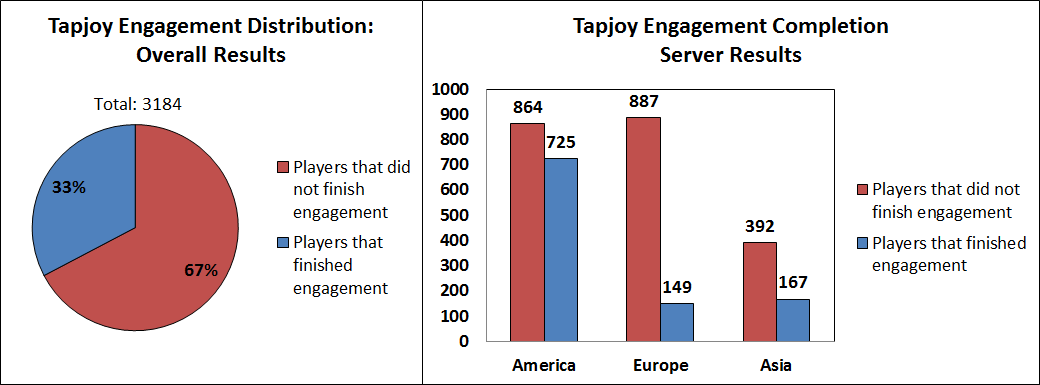
\includegraphics[width=.95\linewidth]{ijhcs14-img/engagement}
		\caption{iCO$_2$ statistics: Engagement.\label{fig:engagement}}
	\end{center}
\end{figure}

\begin{figure}[htb]
	\begin{center}
		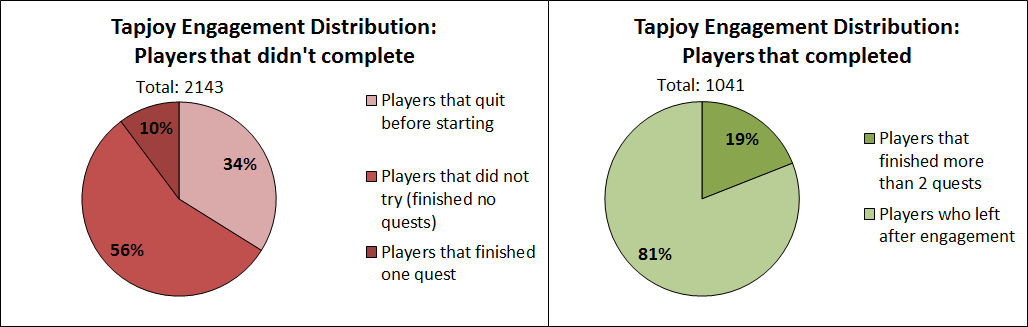
\includegraphics[width=.95\linewidth]{ijhcs14-img/completion}
		\caption{iCO$_2$ statistics: Completion.\label{fig:completion}}
	\end{center}
\end{figure}


\begin{figure}[htb]
	\begin{center}
		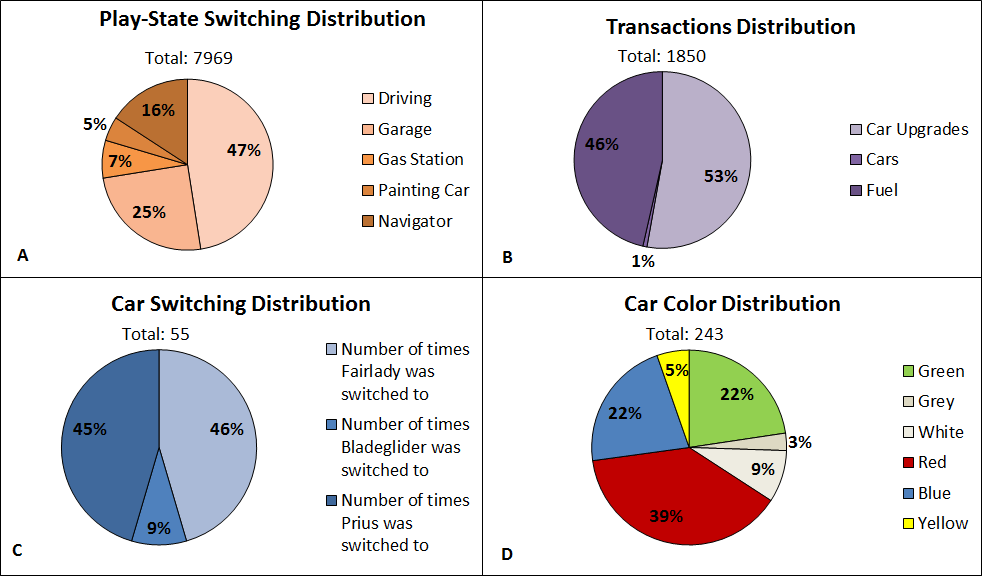
\includegraphics[width=.95\linewidth]{ijhcs14-img/4diagrams2}
		\caption{Various iCO$_2$ statistics.\label{fig:4diagrams}}
	\end{center}
\end{figure}

\begin{figure}[htb]
	\begin{center}
		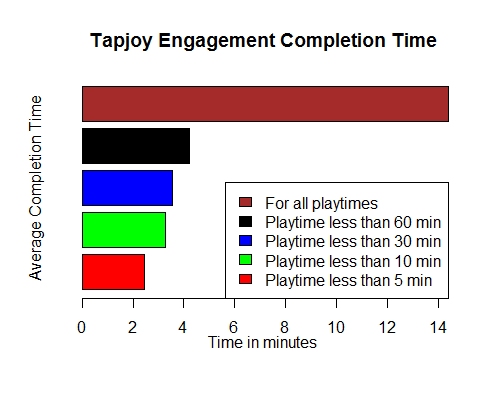
\includegraphics[width=.8\linewidth]{ijhcs14-img/time}
		\caption{iCO$_2$ statistics: Average completion time.\label{fig:time}}
	\end{center}
\end{figure}


Out of a total of 3184 players who played the iCO$_2$, 33\% finished the engagement while 67\% did not, as seen in Figure \ref{fig:engagement}. American players had the highest participation and completion rate, with 725 players finishing the engagement, while 864 did not. European users were most likely to abandon the engagement, with 887 players not finishing and only 149 completing the engagement. 392 Asian users, who were mostly from Japan, did not finish the engagement while 167 did.

Figure \ref{fig:completion} shows the number of players that did not complete the engagement. Out of a total of 2143 users from the second campaign that didn't finish the engagement, 10\% of players finished one quest, 34\% quit before even starting, and 56\% didn't try to finish a quest. Out of the total of 1041 users from the second campaign that completed the engagement, 81\% left after the engagement and 19\% finished more than two quests.


\hlc[green]
{The number of times a determined player logs into the game helps us further understand the way players interact with iCO$_2$, and its re-playability potential. This leads us to the definition of play session as an uninterrupted chunk of play time, it also depicts the number of times the user opened the iCO$_2$ application. The majority of players only played the game once, as we can see on }Figures \ref{fig:playtime_e}, \ref{fig:playtime_as}, and \ref{fig:playtime_a}. 
\hlc[green]{However in the Europe server 21.7\% of the players opened the  game at least twice, that number is 18.8\% for Asia, and 10.2\% for America.}





We can see various iCO$_2$ statistics in Figure \ref{fig:4diagrams}: The play-state switching distribution in Graph A, the transaction distribution in Graph B, the car switching distribution in Graph C and the car color distribution in Graph D. The play-stat was switched a total of 7969 times, mostly towards the driving state (47\%), followed by the garage (25\%), navigator (16\%), gas station (7\%) and lastly painting the car (5\%). Notice that this does not the time spent in a state, but the act of switching from one state to another. In graph B, we can see how users spent their in-game currency. Most of it was spent on car upgrades (53\%) and new cars (46\%), with only 1\% spent on fuel. A total of 1850 transactions were made. Users did not switch their cars very often, only a total of 55 switches occurred as denoted in graph C. Out of these, 46\% of players switched to the ``Fairlady'', 45\% switched to the ``Bladeglider'' and only 9\% switched to the Prius. As for the color distribution, the users preferred a red car by far (39\%), followed by green and blue (22\% each) and the less popular white (9\%), yellow (5\%) and grey (3\%). In total, cars were recolored 243 times.

The average time to complete an engagement is 14 minutes and 42 seconds, as seen in Figure \ref{fig:time}. 
The engagement task was designed so it could be easily completed under 5 minutes. 
\hlc[green]{However when we look at} Figures \ref{fig:playtime_e}, \ref{fig:playtime_as}, and \ref{fig:playtime_a}
\hlc[green]{we can observe that there are players who played for way longer, and even across multiple play sessions. Moreover for every server, the median is set around the 4 minute mark. This brought us to consider some outlier groups when studying the time that took for each player to complete the two quests.}
If we deem all times over 60 minutes outliers, the average completion time drops off to 4 minutes and 23 seconds. It further diminishes to 3 minutes and 53 seconds, if we consider all times over 30 minutes as outliers, to 3 minutes and 26 seconds with outliers over 10 minutes and to 2 minutes and 45 seconds, if we ignore all times over 5 minutes.

\subsection{Clustering}
\label{subsec:clustering}

\hlc[green]{
From a research perspective iCO$_2$ allows the systematic capture of non-supervised data, which enables us to analyze the players' behavior, and understand the overall compliance within the game system.
}
\hlc[green]{
Since iCO$_2$ allows for the practice of eco-driving, supported by the game design discussed in previous sections, we decided to perform clustering to understand how users behaved in term of a profile.
}

\hlc[green]{
Clustering is a form of unsupervised machine learning. It is used to group data into different chunks/profiles, where data from the same group has similar characteristics and data from different groups is dissimilar. Clustering is often applied when the classification details of users are unknown; hence it is a kind of exploratory analysis. No classification standard in advance is needed before clustering.
}

\hlc[green]
{In our work, $k$-means clustering is used} \citep{KMEAN.1979}, 
\hlc[green]{
to obtain player profiles based on the percentage of smooth acceleration they display.
}

\hlc[green]{
In the collected data, the acceleration of the car is between $-$4 m/s$^2$ and 4 m/s$^2$ most of the time, despite the total range being set from $-$6 m/s$^2$ and 6 m/s$^2$.
Akin to
} \cite{prendingeroliveira2014}, 
\hlc[green]{
given the possible acceleration ranges, we define 22 categories for the slope of the acceleration (the changing rate) defined in 
}
Equation \ref{eq:slope_acceleration}, 
\hlc[green]{
starting in $[-inf , -100]$, up to $[100, +inf]$. Giving these categories smooth acceleration is defined as the $[-10, 0]$, and $[0, 10]$ intervals. 
As a preparation for the clustering we found the distribution of the acceleration slope according to those 22 categories for each player. This distribution is already normalized. 
As we are interested on the rate of change of acceleration we removed the idle moments (intervals were the player was idle and the velocity/speed was 0).
}

\hlc[green]{
The sum of squares due to error (SSE) is used to measure the level of convergence of the clusters. The cluster is better the smaller the SSE is. The SSE is calculated by Equation
}
 \ref{eq:sse}.
\begin{equation}\label{eq:sse}
SSE = \sum\limits_{i=1}^{k} \sum\limits_{x \in C_{i}}distance(m_{i},x)
\end{equation}

The SSE can also be used to determine the best number of clusters. We analyzed $k$ from 2 to 15 and selected the $k$ according the elbow criterion \cite{Thorndike.1953}, trying to achieve a low SSE, while using the least amount of clusters in order to explain the data. Here, the appropriate number of clusters $k$ is 4. 

\begin{figure}[htb]
	\begin{center}
		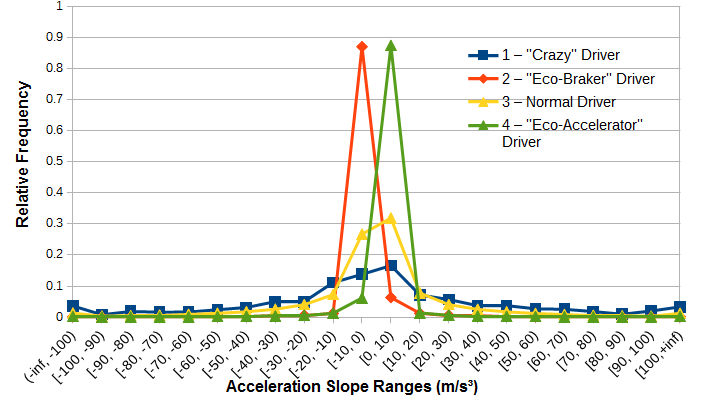
\includegraphics[width=1\linewidth]{ijhcs14-img/kmeansclustering}
		\caption{Clustering of users' driving behavior based on the rate of change of acceleration. In order to analyze the driving behavior we are interested in the relative frequency of smooth acceleration. We consider smooth acceleration the interval $[-10,10)$. We label the cluster 1, ``Crazy`` Driver due to the spread out distribution of the rate of acceleration, which means the users in this cluster performed abrupt brakes, acceleration, and collisions with the world.
			Cluster 2 and 4 on the other hand have a high prevalence of smooth acceleration, even though the cluster 2 focus primarily on smooth braking, and cluster 4 on smooth accelerating, hence the group names ``Eco-Braker`` and ``Eco-Accelerator``. Finally we have a group of players that perform mostly smooth accelerations but still present a considerable amount of abrupt acceleration changes, we label this profile as Normal Drivers. \label{fig:accel-ranges}}
	\end{center}
\end{figure}


Figure \ref{fig:accel-ranges} 
\hlc[green]{
	shows the four cluster profiles we obtained. In order to evaluate the eco-friendliness level of the clusters, we introduce
} Equation \ref{eq:factor-accel-slope}, 
\hlc[green]{which corresponds to the relative frequency on the smooth acceleration bin. The closer this factor is to 1 the more eco-friendly the cluster is.
Detailed results for the clusters obtained are shown in
} Table \ref{T:factors}

\begin{equation}\label{eq:factor-accel-slope}
factor_{eco} = F_{r[-10,10]}
\end{equation}

%sorted table
\begin{table}[!h]
	\renewcommand*{\arraystretch}{1.4}
	\caption{This table presents a summary of the clusters. Here we can see discriminated the relative frequency of smooth acceleration for each cluster; the $factor_{eco}$. Moreover the majority of players fits the Normal Driver profile with a considerable amount of smooth acceleration, mixed with abrupt changes. The percentage of users classified as ``Crazy`` (8.08\%) is less that the sum of the two eco-friendly clusters (``Eco-Brakers`` and ``Eco-Accelerators``), combined. }
	\begin{center}
		\begin{tabular}{c|c|c|c}
			Cluster & $factor_{eco}$ & \% of Users & Cluster Label \\
			\hline
			1 &	 0.30
			& 8.08  & ``Crazy`` Driver  \\
			
			2 & 0.93
			& 7.6  &  ``Eco-Braker`` Driver \\
			
			3 &	 0.59
			& 73.1  &  Normal Driver  \\
			
			4 & 0.94
			& 11.2  &  ``Eco-Accelerator`` Driver \\
		\end{tabular}
	\end{center}
	\label{T:factors}
\end{table}


\hlc[green]{
The most distinguishable characteristic between clusters is the proportion of smooth acceleration (between $[-10, 10[$), we can clearly establish that there is a type of player who spends most of his playing time accelerating and braking very smoothly. This player profile is illustrated on the clusters labeled as ``Eco-Braker`` Driver and  ``Eco-Accelerator`` Driver, 
}(Figure \ref{fig:accel-ranges}),
\hlc[green]{ we call these players under these classifications Eco-Drivers or Eco-Friendly. The main difference between these clusters is the emphasis on accelerating versus the emphasis on braking. These two clusters combined amount for 18.8\% of the players.
}

\hlc[green]{
Cluster 3, labeled as Normal Drivers, aggregates the vast majority of the drivers and shows an intermediate percentage of time on the smooth acceleration interval (73.1\%). Players in this cluster perform a considerable percentage of smooth accelerations 58.6\%. These players complied with the game's eco-driving stance most of the time.
}

\hlc[green]{
We also verified that there is a driver profile, classified under cluster 1, characterized by very extreme variations in acceleration. This is the cluster with the least prevalence on the smooth acceleration zone (8.08\%). Users in this cluster often engaged in abrupt braking, collisions with the world, high acceleration, making them not comply with the game eco-driving philosophy. We call this cluster the eco-unfriendly or ``Crazy`` drivers. 
This disruptive behavior profile (cluster 1), was the least prevalent among the iCO$_2$ drivers (around 8.08\% of users).
It is important understand that the main benefit of clustering the driving behavior is the fact that enables understanding our players under profiles obtained from the data (using $k$-means clustering).
}






\subsection{Types of Drivers}
\hlc[green]{
After having our players classified according to the clusters in the previous section it's interesting  looking for insights on how that classification might affect other game activities.
}

\hlc[green]{
For example the correlation between driver type and the car color picked by the player. We measured the probability between painting a car a determined shade and being “Eco-unfriendly”.
“Eco-unfriendliness is characterized by the levels/ranks the $factor_{eco}$ parameter on} Table \ref{T:factors} 
\hlc[green]{this enables us to order our clusters from the most eco-friendly to the least eco-friendly: Cluster 4 $<$ Cluster 2 $<$ Cluster 3 $<$ Cluster 1, or ``Eco-Accelerator``  $<$ ``Eco-Braker`` $<$  Normal $<$ ``Crazy``. 
}
\hlc[green]{
In order to find associations between the data we use Kendall correlation coefficient, which enables us to understand the relationship between the ranks of the variables. We performed this analysis for every car color, for each server.
For Kendall correlation coefficient consider that, in absolute value, correlations less than 0.10 are very weak, between 0.10 and 0.19 are considered weak, between 0.20 and 0.29 moderate, and when we have correlations greater or equal than 0.30 we consider them strong.

We noticed that the different servers having distinct biases for the color chosen and how eco-unfriendly a user is according to his profile obtained by clustering the acceleration rate.   
}

For example painting the a car green tended to be more associated with being eco-friendly on both Europe with Kendall correlation coefficients of -0.22, in America the association is weak -0.11, while in the Asia dataset, despite the association being weak, it points to a weak relation towards eco-unfriendlyness with a Kendall coefficient of 0.14. Here we can only say that the European server has a slight bias towards being more eco-friendly.

Choosing the color blue for the car is associated with being more eco-unfriendly in Europe (0.60), and Asia (0.30), while having no apparent relation in America (0.001).
The Red color also seems to have no impact in the America dataset (0.03), while being associated with being more eco-friendly both in Asia(-0.45) and having a slight association with eco-unfriendliness in Europe (0.26).

The color gray seems to be associated with being more eco-unfriendly in a weak way in every server with the correlation coefficients being greater than 0.11 for Asia, up to Europe with 0.17. The color yellow has a moderate association with being more eco-unfriendly in Asia (0.20).

%
% The joint distributions for the chosen color and the driver type according to our driving style clustering can be observed in} Tables \ref{T:colour_correlation_europe}, \ref{T:colour_correlation_asia}, and \ref{T:colour_correlation_america}.



\textcolor{black}{
We also analyzed the correlation of the quest completion rate and number of quests started and the driver type. And we found that the quest completion rate seems not to have any relationship with being more eco-friendly. 
However when we consider the number of quests started and the number of quests completed 
particularly in every server there is a weak association with between being more eco-unfriendly and completing quests, and starting quests (correlation coefficients for the servers between 0.14 and 0.17 ). 
}
\textcolor{black}{
The number of times a player refueled does not seem to have a relationship with being more of less Eco-friendly within the Europe data set (0.07). On the other hand the America and Asia data sets show a relationship between these the frequent refueling and being more eco-unfriendly, ( Asia with a Kendall Correlation Coefficient of 0.15, and America with 0.23), albeit only America displays a moderate association.
}





\hlc[green]{
As discussed in the }
Section \ref{sec:platform}
\hlc[green]{
, users have access to 5 different activities in the game. They can drive, go to the garage, gas station, use the navigator tool to plan their routes, or go to the car painter. 
We performed $k$-means clustering to understand how the users spend their time within the game, and what activities they engage in. We aim at extracting profiles of a time distribution of how users spend their time in the game.
For this clustering we considered users who played more than 4 minutes. Because this is the median time it took to finish the Tapjoy engagement. 
} 

{ 
Using the 'elbow' heuristic to minimize the Sum of squares due to error (Equation \ref{eq:sse}), we found 4 activity distribution profiles represented on Table \ref{T:cluster_activities}.  
}
\begin{table}[!h]
	\renewcommand*{\arraystretch}{1.2}
	\caption{Time distribution of Activities cluster means. We obtained 4 profiles on how the users spend their play time. Our clusters 1 and 2 are labeled as "Refuelers", and "In-Game Explorers", these players spend a great part of their time doing in-game activities others than driving. Then we have a class of drivers that practically only drives, the center of mass of this cluster has a driving percentage of 97\%; we call this group ""Pure Drivers". Then we have a class of users that engage primarily on driving, while doing other in-game activities, we label this profile as "Drivers".   }
	\begin{center}
		\begin{tabular}{c|c|c|c|c|c}
			Cluster Number	& Gas Station &	Garage &	Navigator &	Driving &	Car Painter 	\\
			1 - "Refuelers" &	0.29 &	0.09 &	0.04 &	0.55 &	0.03\\
			2 - "In-Game Explorers" &	0.03 &	0.24 &	0.02 &	0.52 &	0.18 \\
			3 - "Pure Drivers" &	0 &	0.01 &	0.01 &	0.97 &	0  \\
			4 - "Drivers" &	0.03 &	0.12 &	0.04 &	0.78 &	0.03   \\
		\end{tabular}
	\end{center}
	\label{T:cluster_activities}
\end{table}

\hlc[green]{
As expected driving takes up the majority of time spent in the game. Moreover the majority of players, only engages on the driving aspect of the game as we can see on the Cluster 3, which we labeled as "Pure Drivers". 
}

In Figure \ref{fig:activity_driving} we can also notice that being only interested on the driving aspect of the game is prevalent across every type of driver. However the players selected for the driving clustering (those who played the longest), also manifested interest in exploring every activity iCO$_2$ has to offer, a profile illustrated by the activity cluster 2.

Surprisingly the activity profile associated with more time spent at the gas station has a high prevalence among the eco-friendly. Two possible hypotheses to explain this behavior is the fact that the more eco-friendly users were more conscious of their fuel tank data at all time. The cluster labels as ''Refuelers'' is also one of which has more time spent on Route planning (Navigator), and manifested curiosity to try the various activities the game has to offer. On the other hand, and not so surprisingly, those players labeled as "Crazy Drivers" also had more tendency to be "Refuellers" (35\%). It's curious that this activity profile tends to be more prevalent either with those who comply strictly with the game goal. 

The probability of being a driver (a user that spends almost all of his time driving), while still participating in other game activities, tends to increase with being a less eco-friendly driver.

Normal drivers had the highest percentage of "In-game Explorers".


%\begin{table}[!h]
%	\renewcommand*{\arraystretch}{1.2}
%	\caption{Joint distribution of player driving profile and in-game activity profile.}
%	\begin{center}
%		\begin{tabular}{c|c|c|c|c}
%			& Activity & Activity& Activity& Activity \\
%			Driving Behavior	& Cluster 1 &	Cluster 2 &	Cluster 3 &	Cluster 4 	\\
%			Cluster 1 &	0.010 &	0.015 &	0.013 &	0.005 \\
%			Cluster 3 &	0.003 &	0.010 &	0.008 &	0.010 \\
%			Cluster 4 &	0.028 & 0.268 &	0.130 &	0.0251  \\
%			Cluster 2 &	 0.058 &	 0.226 &	0.143 & 0.050  \\
%		\end{tabular}
%	\end{center}
%	\label{T:joint_activity_driving}
%\end{table}

\begin{figure}[htb]
	\begin{center}
		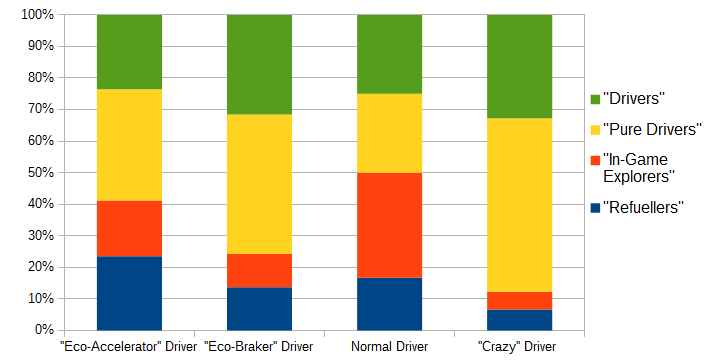
\includegraphics[width=.8\linewidth]{ijhcs14-img/cluster_activities_driver_types}
		\caption{Distribution of the activity clusters among the user's driving profile.\label{fig:activity_driving}}
	\end{center}
\end{figure}



\subsection{Analysis of players' eco-friendliness over time }
\label{subsec:eco-friendliness_over_time}

In this section, the aim of research is to test the hypothesis that the players who appear to be less eco-friendly in the beginning of their play-time improve as they play further. The approach is to select the players who played more than a certain amount of time and calculate the variation of the probabilities of them having smooth acceleration in discrete uniform time-intervals. 

To implement this approach, four different play-times of 7, 8, 9 and 10 minutes are chosen. The reason behind the choice of these playtimes is that we wanted a player to drive for a reasonably longer period so that their performance can be tested. Then for each group of players that correspond to a different play-time, a clustering based on the probability of their jerk distribution(refer Equation~\ref{eq:factor-accel-slope}) is made so as to form the concepts of driver-types after a formal train session of first two minutes ends. These conceptual driver-types are named as "Eco-friendly", "Gentle", "Normal" and "Crazy". Figure~\ref{fig:evolution} shows: a) four different groups of players filtered according to their net driving time  a)the number of players who fall into those groups b) the distribution of players within the four clusters of driver-types and d) time-varying distribution of the eco-friendliness of different driver types. 


\begin{figure}[!htb]
	\centering
	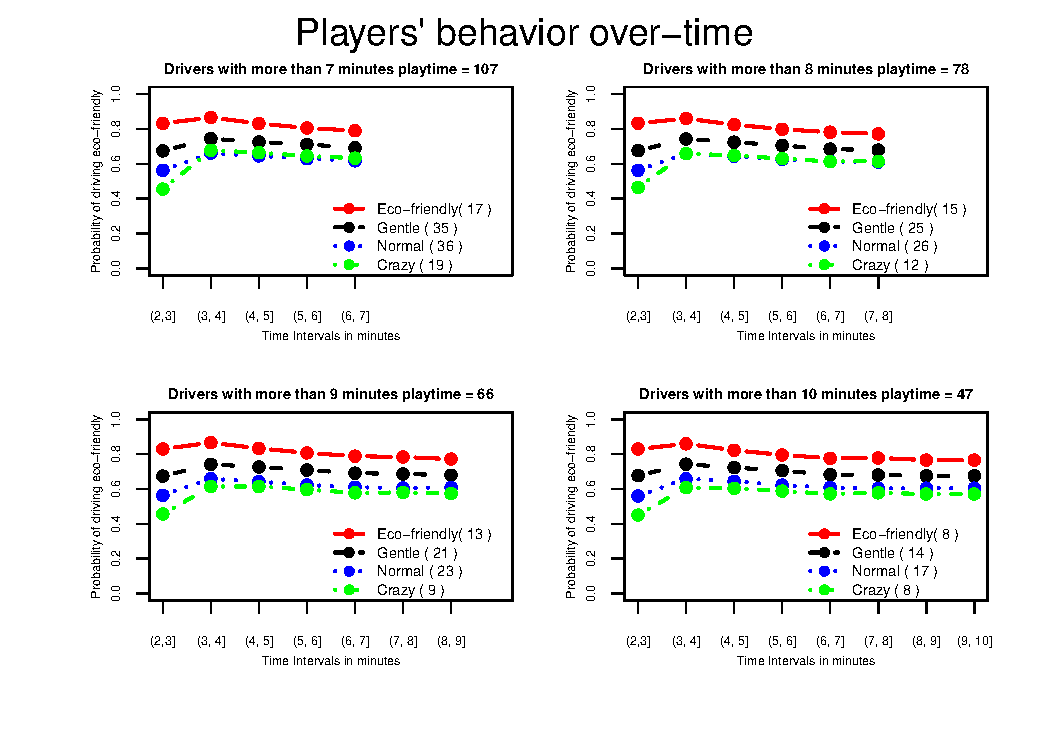
\includegraphics[trim = 10mm 13mm -15mm 10mm, width=20.0cm,height=18.0cm]{ijhcs14-img/Evolution.pdf}
	\caption{The analysis of driving behavior of players in term of its eco-friendliness is determined. A total of 2045 users were selected. The players are filtered into \textit{four} groups according to their net driving time. For each group, the players are clustered into \textit{four} clusters after training their driving with the simulator for first two minutes. Then their probability of having smooth acceleration within a certain time interval is calculated. The graphs show that for all the four groups, the \emph{crazy} drivers tend to perform eco-friendlier over time and match those termed as \textit{gentle} post-training. 
	}
	\label{fig:evolution}
\end{figure}

Figure~\ref{fig:evolution} shows that "Gentle" drivers among all the driver-types contain the biggest chunk of players across all the four groups whereas "Crazy" drivers have the smallest share. The share of "Gentle" drivers is 32.7\%, 32.05\%, 31.81\% and 29.78\% for the players who played more than 7 minutes, 8 minutes, 9 minutes and 10 minutes respectively, while the share of "Crazy" drivers is 17.75\%, 15.5\%, 13.6\% and 17\%. The data shows that the order of share of players according to the driver-types across all the groups is:  "Crazy" \textless "Normal" \textless "Gentle" \textless "Eco-friendly". This suggests that after due to the result of training (done for first 2 minutes of playtime), only a few drivers continue to drive is least eco-friendly way. 

To analyze the multi-plot figure~\ref{fig:evolution}, we set a convention to read it by row. For all the plots, it can be seen that the eco-friendliness of the "Crazy" drivers improves significantly over time and becomes comparable with that of the "Normal" drivers. The eco-friendliess of "Gentle" drivers between the start and end of playtime has also increased. However, even the  the high-performance users i.e. the "Eco-friendly" ones continue to maintain their edge over other driver-types, in absolute terms they tend to deteriorate over time. This could be due to several factors like prioritizing the quests. The nature of quests require a player to accelerate and decelerate to stop the car, which will increase player's distribution in non-smooth acceleration zones, this a fluctuation in eco-friendliness is quite likely. Another reason could be simple fatigue while continuing to play the game with sophisticated control. It can be noticed that for all the four driver-types across all the four groups, the peak improvement occurs between 3 minutes to 4 minutes of play-time. For the sake of discussion, we would like to argue that this finding is correlated with the fact that the median time for performing two quests i.e. having an engagement is 4 minutes and players get paid only when they finish an engagement. Thus, it can be hypothesized that players' motivation to "perform" decreases once they get paid and also because in-game currency  enables them to make transactions like car upgrades, buying cars and the fuel etc. thus drawing attention. 

Overall, our results validate the hypothesis that the players who appear to be less eco-friendly in the beginning of their play-time improve as they play further. 

\section{This is a TEST}
{
Later should be deleted. }

\section{Conclusions} \label{sec:conclusions}

In this paper, we describe iCO$_2$, a game-like simulation platform for collecting large-scale driving behavior data (and other data on users' in-game activities, such as upgrading the user's car), 
\hlc{arg1}{arg2} while offering a virtual environment for the practice of eco-driving. 
As a research tool, iCO$_2$ can be seen as a Human Computation system where humans provide driving behavior. This allows us to better understand how users interact with a game that motivates them to drive eco-friendly. In this way, our system is related to other activities aimed at attracting users' work, such as Games with a Purpose or crowdsourcing.

We have described our newest version of iCO$_2$ that extends the previous version \citep{prendingeroliveira2014} by a quest system and a ``garage'' to improve the capabilities of the player's vehicle.

The core contribution is our iCO$_2$ campaign. Since our simulation platform is developed as a mobile app, we could use a mobile games promoter to attract users to our game. Fortunately, data of more than 3000 users could be collected in about one week. We were interested both in results about eco-driving behavior and results about the usage of our system.

If we consider everyone who played the game for more than 30 minutes as an outlier, we could engage the average user for almost in our campaign. Almost 1/5 of the users continued to play the game after the required two quests were completed.
The usage data also revealed some interesting details about users' in-game behavior, such as play-state switching, transaction, car switching and car color switching.
The most frequently active game state was driving (47\%), most in-game currency was spent on car upgrades (53\%), players switched evenly to the ``Fairlady'' as well as ``Bladeglider'' car models (45\%/46\%, respectively) and the most used color for cars was red (39\%). Such results can be used to inform the developer to design a better game.

\hlc[green]{
The analysis of driving behavior (change of the rate of acceleration) suggests that drivers can be grouped into four clusters. These clusters have different eco-level factors and help us group our drivers into three categories "Eco-Driver" (18.8\%), "Normal Drivers" (73.1\%). A small percentage of players (8.08\%) exhibits very abrupt changes in acceleration, nevertheless iCO$_2$ players spent most of their time performing smooth accelerations, with the "Normal Drivers" cluster average of smooth accelerations being 58.6\%.
}

The campaign and its analysis is an important step towards understanding players of mobile games that have a `serious' aspect, such as sustainable behavior. The next is to use the information of player types (eco-unfriendly, ``crazy'', etc) and classify the user's behavior in real-time. This classification can be used to alert the user during the game.

Future work will also try to increase the re-playability of the game to be able collect data of users over time. This opens up entirely new ways of feedback mechanisms to users as we may learn the user's behavior and reactions.


\section{Acknowledgments}
We are grateful to Klaus Bruegmann for coordinating the game design of iCO$_2$, and Tristan Imbert and Kugamoorthy Gajananan for helping with the preparation of the campaign.
This work is partly supported by a Kaken B grant from the Japan Society for the Promotion of Science and by Portugal’s Fundação para a Ciência e a Tecnologia, under project
PEst-OE/EEI/LA0021/2013


%% The Appendices part is started with the command \appendix;
%% appendix sections are then done as normal sections

\section*{References}
\bibliographystyle{elsarticle-harv}
\bibliography{ijhcs-2014}

%\appendix

%\section{Additional Tables}\label{app:tables}
%This section contains additional tables of our findings.

%sorted table
%\begin{table}[!h]
%\renewcommand*{\arraystretch}{1.4}
%\caption{Example of driving behavior data.}
%\begin{center}
%\begin{tabular}{c|c|c|c}
%Timestamp & Position $X$ & Position $Y$ & Position $Z$ \\
%\hline
%1 & 299.5657 & 1.241717 & 0.065165 \\

%2 & 299.2299 & 3.699343 & 0.065120  \\

%3 & 299.2299 & 3.699343 & 0.06512 \\

%4 & 298.8777 & 6.260628 & 0.066202 \\

%5 & 298.8777 & 6.260628 & 0.066202 \\

%6 & 298.7033 & 7.509112 & 0.066517 \\

%\ldots &  \ldots & \ldots & \ldots \\

%2635 & 300.7204	& $-$6.95397 & 0.064981 \\

%2636 & 300.8299	& $-$7.72201 & 0.065020 \\

%2637 & 300.8299	& $-$7.72201 & 0.065020 \\

%2638 & 301.0301	& $-$9.08316 & 0.065068 \\

%2639 & 301.1052	& $-$9.57525 & 0.065062
%\end{tabular}
%\end{center}
%\label{T:drivingdata}
%\end{table}


%sorted table
%\begin{table}[!h]
%\renewcommand*{\arraystretch}{1.4}
%\caption{Acceleration ranges and example values of user in those ranges.}
%\begin{center}
%\begin{tabular}{c|c}
%Range & Value \\
%\hline
%[$-$infinite, $-$5.00] & 15.5022 \\

%[$-$5.00, $-$4.00]	& 5.0364 \\

%[$-$4.00, $-$3.00]	& 11.1235 \\

%[$-$3.00, $-$2.00]	& 4.0027 \\

%[$-$2.00, $-$1.00]	& 21.825 \\

%[$-$1.00, 0.00]	& 20.3731 \\

%[0.00, 1.00]	& $-$0.19349 \\

%[1.00, 2.00]	& $-$0.01021 \\

%[2.00, 3.00]	& 3.7433 \\

%[3.00, 4.00]	& 3.5839 \\

%[4.00, 5.00]	& 4.5173 \\

%[5, +infinite]	& 13.6953 \\
%\end{tabular}
%\end{center}
%\label{T:acceleration}
%\end{table}


%sorted table
%\begin{table} [!h]
%\renewcommand*{\arraystretch}{1.4}
%\caption{Velocity ranges and example values of user in those ranges.}
%\begin{center}
%\begin{tabular}{c|c}
%Range & Value \\
%\hline
%[0.00, 30.00] &	     0.113387 \\

%[30.00, 60.00] &	$-$0.03678 \\

%[60.00, 90.00] &	$-$0.12182 \\

%[90.00, 120.00] &	$-$0.05689 \\

%[120,  +infinite] &	$-$0.05036
%\end{tabular}
%\end{center}
%\label{T:velocity}
%\end{table}




%\section{Additional Charts}
%% \label{}
%This section contains additional charts from our campaigns.

%\begin{figure}[ht]
% \centering
% \subfigure[Campaign requirements]{
%  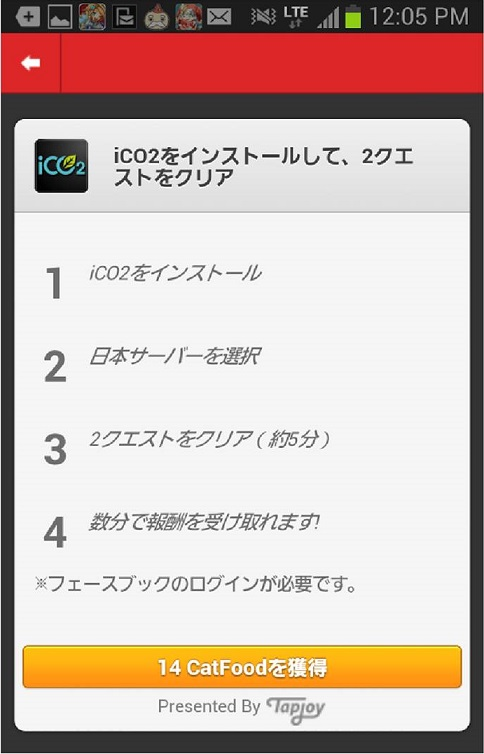
\includegraphics[scale=0.5]{ijhcs14-img/tapjoy}
%   \label{fig:requirements}
%   }
% \subfigure[Display of iCO$_2$ in game list]{
%  
\includegraphics[scale=0.55]{ijhcs14-img/gamelist}
%   \label{fig:gamelist}
%   }
% \label{fig:tapjoy}
% \caption[Tapjoy campaign]{%
%  Tapjoy campaign
%  }
%\end{figure}


%\clearpage % Start a new page

%\setstretch{1.5} % Set the line spacing to 1.5, this makes the following tables easier to read

%\section{Abbreviations}\label{app:abbreviations}
%\listofsymbols{ll} % Include a list of Abbreviations (a table of two columns)
%\begin{tabular}{ l | l }
%	\textbf{3D} & \textbf{3} \textbf{D}imensional \\
%	\textbf{DiVE} & \textbf{Di}stributed \textbf{V}irtual \textbf{}Environments \\
%	\textbf{ESP} & \textbf{E}xtra\textbf{s}ensory \textbf{P}erception  \\
%   \textbf{GWAP} & \textbf{G}ames \textbf{W}ith \textbf{A} \textbf{P}urpose \\
%    \textbf{iOS} & \textbf{i}Phone \textbf{O}perating \textbf{S}ystem \\
%    \textbf{MMO} & \textbf{M}assive \textbf{M}ultiplayer \textbf{O}nline \\
%    \textbf{MMOG} & \textbf{M}assive \textbf{M}ultiplayer \textbf{O}nline \textbf{G}ame \\
%    \textbf{SSE} & \textbf{S}um of \textbf{S}quares due to \textbf{E}rror \\
%\end{tabular}


%\begin{figure}[htb]
%\begin{center}
%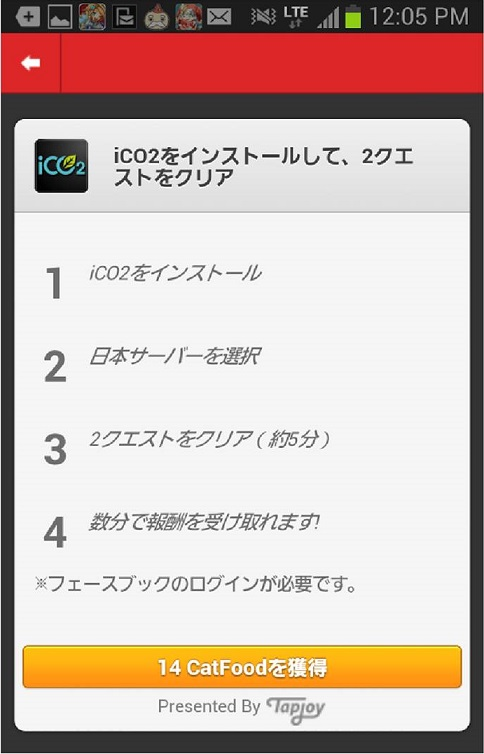
\includegraphics[width=.4\linewidth]{ijhcs14-img/tapjoy}
%\caption{Requirements of the Tapjoy campaign.\label{fig:requirements}}
%\end{center}
%\end{figure}

%\begin{figure}[htb]
%\begin{center}
%
\includegraphics[width=.4\linewidth]{ijhcs14-img/gamelist}
%\caption{Presentation of iCO$_2$ campaign in game list.\label{fig:gamelist}}
%\end{center}
%\end{figure}

\appendix
\section{Play Sessions}
\begin{figure}[htb]
	\begin{center}
		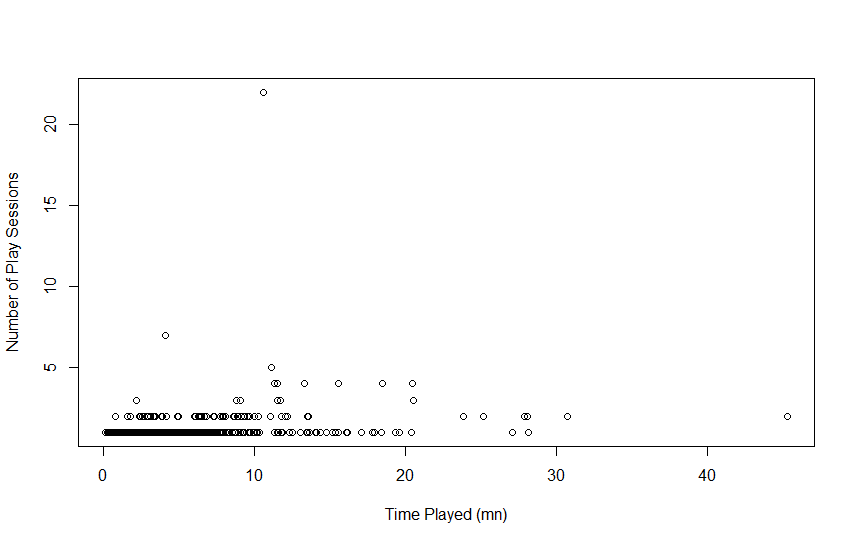
\includegraphics[width=.8\linewidth]{ijhcs14-img/playsessions_europe}
		\caption{Distribution of play sessions by total play time for Europe.\label{fig:playtime_e}}
	\end{center}
\end{figure}

\begin{figure}[htb]
	\begin{center}
		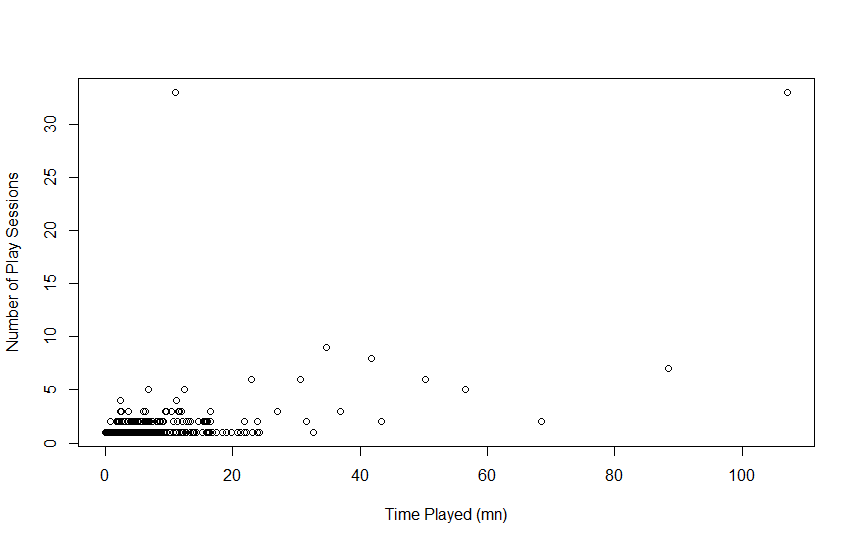
\includegraphics[width=.8\linewidth]{ijhcs14-img/playsessions_asia}
		\caption{Distribution of play sessions by total play time for Asia.\label{fig:playtime_as}}
	\end{center}
\end{figure}

\begin{figure}[htb]
	\begin{center}
		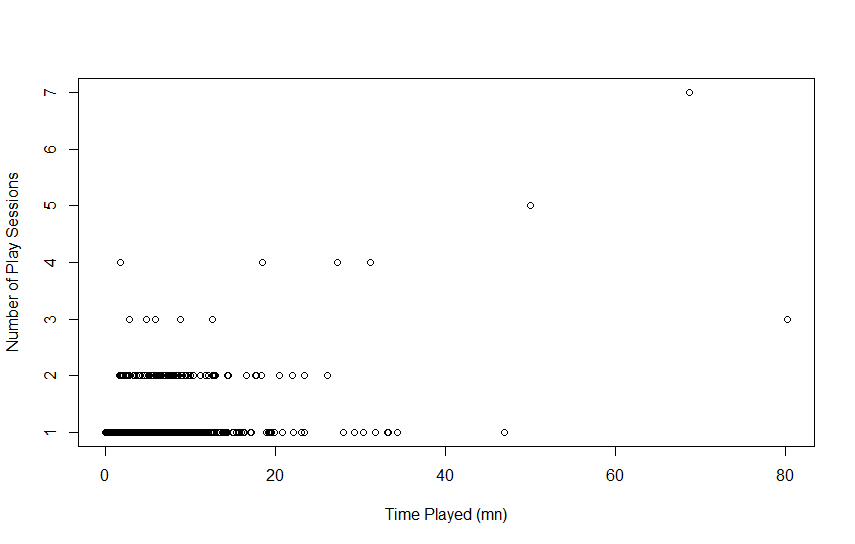
\includegraphics[width=.8\linewidth]{ijhcs14-img/playsessions_america}
		\caption{Distribution of play sessions by total play time for America.\label{fig:playtime_a}}
	\end{center}
\end{figure}

%\section{Driving Behavior and Chosen Car Color}
%
%\begin{table}[!h]
%	\renewcommand*{\arraystretch}{1.2}
%	\caption{Joint distribution of player profile and chosen car color for Europe.}
%	\begin{center}
%		\begin{tabular}{c|c|c|c|c}
%			Color	& Cluster 1 &	Cluster 3 &	Cluster 4 &	Cluster 2 	\\
%			Blue &	0.091 &	0.045 &	0.000 &	0.045 \\
%			Gray &	0.000 &	0.000 &	0.000 &	0.091  \\
%			Green &	0.000 & 0.000 &	0.091 &	0.045  \\
%			Red &	 0.000 &	 0.000 &	0.227 & 0.227  \\
%			White &	0.000 &	0.000 &	0.091 &	0.045  \\
%			Yellow &	0.000 &	0.000 &	0.000 & 0.000 \\
%		\end{tabular}
%	\end{center}
%	\label{T:colour_correlation_europe}
%\end{table}
%
%\begin{table}[!h]
%	\renewcommand*{\arraystretch}{1.2}
%	\caption{Joint distribution of player profile and chosen car color for Asia.}
%	\begin{center}
%		\begin{tabular}{c|c|c|c|c}
%			Color	& Cluster 1 &	Cluster 3 &	Cluster 4 &	Cluster 2 	\\
%			Blue &	0.033 &	0.067 &	0.000 &	0.067 \\
%			Gray &	0.000 &	0.033 &	0.000 &	0.133  \\
%			Green &	0.100 & 0.000&	0.033 &	0.167  \\
%			Red &	 0.000 &	 0.000 &	0.100 & 0.167  \\
%			White &	0.000 &	0.000 &	0.000 &	0.067  \\
%			Yellow &	0.000 &	0.033 &	0.000 & 0.000 \\
%		\end{tabular}
%	\end{center}
%	\label{T:colour_correlation_asia}
%\end{table}
%
%
%\begin{table}[!h]
%	\renewcommand*{\arraystretch}{1.2}
%	\caption{Joint distribution of player profile and chosen car color for America.}
%	\begin{center}
%		\begin{tabular}{c|c|c|c|c}
%			Color	& Cluster 1 &	Cluster 3 &	Cluster 4 &	Cluster 2 	\\
%			Blue &	0.043 &	0.000 &	0.130 &	0.043 \\
%			Gray &	0.000 &	0.000 &	0.000 &	0.0436  \\
%			Green &	0.000 & 0.000 &	0.130&	0.087  \\
%			Red &	 0.000 &	 0.043&	0.217 & 0.174  \\
%			White &	0.000 &	0.000 &	0.000 &	0.043  \\
%			Yellow &	0.000&	0.000 &	0.043 & 0.000 \\
%		\end{tabular}
%	\end{center}
%	\label{T:colour_correlation_america}
%\end{table}

\end{document}
%%% Local Variables:
%%% coding: euc-japan 